% -*- mode: LaTeX; coding: utf-8; -*-

\thispagestyle{plain}
\section{Введение}
Изучение природы взаимодействия ядерной материи немыслимо без методов
регистрации частиц. Эти методы возникали и совершенствовались
по мере развития ускорительной техники, теоретических воззрений, увеличения
типов и энергии частиц и т.д. Во времена открытия лучей Рентгена
использовались обычные фотографические пластинки. Такие же "<детекторы">
способствовали открытию радиоактивности и сыграли важную роль в атомной
и ядерной физике.

Однако, по мере развития физики частиц, усложнялись требования к методам
наблюдения траекторий отдельных частиц, определению их природы. Это привело
к изобретению различного рода детекторов --- процессу, который продолжается
и по сей день. Появились камеры Вильсона, диффузионные и пузырьковые
камеры.

На первых порах эти приборы, а также специально изготовленные ядерные
фотоэмульсии использовались в наблюдении взаимодействий в космических лучах.
Эти редкие и беспорядочно направленные частицы из космоса создавали
трудности для регистрации их взаимодействий с веществом. Возникла проблема
сооружения "<космотронов"> --- так стали называть ускорители частиц высоких
энергий. Эти приборы развивались по своим законам. Физики стремились получить
всё более и более высокоэнергичные частицы.

Эксперименты на современных ускорителях требуют "<расшифровки"> сложных
событий, включающих сотни и тысячи вторичных частиц. Соответственно
усложнились и детекторы для их наблюдения и измерений параметров заряженных
частиц. Нашей задачей является сделать некоторый обзор средств наблюдения
вторичных частиц с акцентом на газовые координатно-трековые детекторы,
которые являются непременной составляющей всех экспериментальных установок.

Сначала рассматриваем физические процессы, происходящие при прохождении
частиц через вещество, которые позволяют регистрировать следы ионизирующих
частиц и без которых невозможно понять работу любого детектора. Затем
коротко останавливаемся на использовавшихся до последнего времени трековых
приборах различного типа с коротким анализом их преимуществ и недостатков.

Последний раздел реферата посвящён принципу работы наиболее широко
используемым в физических установках многопроволочным пропорциональным
и дрейфовым камерам.

\section{Взаимодействие частиц с веществом}
Принцип работы любого детектора связан с характером взаимодействия
частицы с веществом данного прибора. Заряженная частица или гамма квант,
проходящая  через материю, может потерять свою энергию частично или
полностью в зависимости от типа взаимодействия.

Если не считать очень слабого гравитационного взаимодействия, существуют
три вида взаимодействия излучения с веществом:
\begin{description}
\item[сильное (ядерное)] наиболее интенсивное. Оно может
  проявляться как в процессах непосредственного взаимодействия, так и
  в~процессах распада ядер или частиц. Сильные процессы характеризуются
  очень большими сечениями и коротким действием сил.
\item[электромагнитное] второе по интенсивности. ~Определяет
  взаимодействие заряженных частиц и $\gamma$-квантов. Дальнодействующий
  характер сил и значительно большее число электронов в веществе, чем
  атомных ядер, определяет доминирующую роль в процессе взаимодействия
  излучения с атомами.
\item[слабое] кроме процессов распада, оно может проявляться и в
  процессах захвата нейтрино (антинейтрино) нуклоном, однако сечение таких
  процессов очень малое.
\end{description}

Главную роль при прохождении заряженных\footnote{Нейтроны
  регистрируются по вторичным заряженным частицам, возникающим благодаря
  их сильному взаимодействию с ядрами.}
%можно регистрировать косвенно, сначала они должны образовать вторичные
%заряженные частице благодаря сильному взаимодействию с ядрами.}
частиц и $\gamma$-квантов через вещество играют электромагнитные
взаимодействия. Правда, частицы могут взаимодействовать и с атомными
ядрами, однако основные потери энергии и эффекты рассеяния определяются
взаимодействием с атомными электронами. Поэтому интересующие нас
процессы скорее подчиняются атомной, а не ядерной физике.

По механизму прохождения через вещество частицы можно разделить
на следующие группы:
\begin{itemize}
\item[-] тяжёлые заряженные частицы ($p,~d,~\alpha$,~ ионы, \dots)
\item[-] лёгкие заряженные частицы ($e^\pm$)
\item[-] гамма---излучение
\item[-] нейтроны
\end{itemize}
\clearpage
Разные процессы взаимодействия частиц не позволяют нам рассматривать их
все вместе. Рассмотрим отдельно главные виды взаимодействий со средой
заряженных частиц (ионизационные потери, тормозное, черенковое излучение,
многократное рассеяние), $\gamma$-квантов (фотоэффект, Комптон эффект,
образование электрон---позитронных пар) и в~конце кратко обсудим
взаимодействие нейтронов с веществом.

\subsection{Ионизационные потери энергии}
Основные потери энергии быстрых тяжёлых заряженных частиц происходят
в~результате кулоновского взаимодействия при столкновениях с~атомными
электронами. Заряженная частица либо возбуждает атом, либо ионизирует.
Такие процессы обычно называют ионизационными потерями или
торможением.

Средние потери энергии $-dE$ на единицу пути $dx$ для заряженных тяжёлых
$(m\gg m_e)$ частиц определяются формулой Бете---Блоха \cite{pdg}:
\[
-\frac{dE}{dx}=Kz^2\frac{Z}{A}\frac{1}{\beta^2}
\Biggl[\frac{1}{2}\ln\frac{2m_ec^2\beta^2\gamma^2T_{max}}{I^2}-\beta^2-\frac{\delta}{2}\Biggr],
\]
где
\begin{itemize}
\item $K=4\pi N_Ar_e^2m_ec^2$ = 0.307075 MeV/(g~cm$^{-2}$);
\item $z,~\beta = v/c$ - заряд и скорость налетающей частицы;
\item $Z, A$ - атомный номер и атомный вес среды;
\item $T_{max}$ - максимальная кинетическая энергия переданная электрону;
\item $I$ - средний ионизационный потенциал поглощающего вещества,
  приблизительно равный $I\cong 16~Z^{0.9}$ eV;
\item $\delta$ - параметр учитывающий релятивистский эффект поляризации
  среды пролетающей через неё релятивистской частицей (определяется
  экспериментально).
\end{itemize}
При анализе реальных экспериментов толщину вещества измеряют не
в~единицах длины, а величиной $\rho dx$, где $\rho$ плотность поглотителя.
Так называемые удельные потери энергии
$\frac{dE}{d(\rho x)}=\frac{1}{\rho}\frac{dE}{dx}$ принято приводить
в единицах $\frac{MeV}{g~cm^{-2}}$. Удельные ионизационные потери энергии
слабо зависят от свойств материала. На рис.~\ref{fig:loss1} хорошо виден
общий характер указанной зависимости.
\begin{figure}[h]\center
  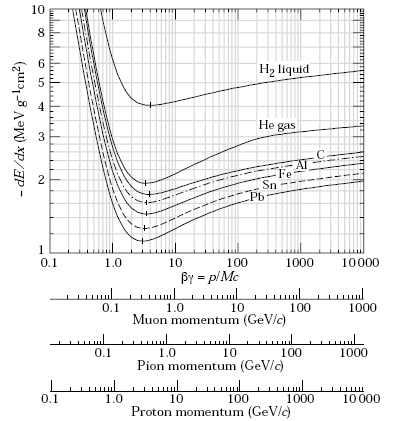
\includegraphics[scale=0.77]{loss1}
  \caption{Зависимость удельных потерь энергии в водороде, гелии,
    углероде, алюминии, железе, олове и свинце от импульса мюона,
    пиона и протона.}
  \label{fig:loss1}
\end{figure}

Формула приближенная, однако это приближение вполне достаточно (точность
порядка нескольких процентов). Уравнение несправедливо\footnote{
  Добавляется параметр, который уменьшает ионизационные потери за счёт
  связи электронов на K и L оболочках атомов.} для медленных частиц,
скорость которых сравнима со скоростями атомных электронов.
При этих скоростях потери энергии пропорциональны~$\beta$. С увеличением
скорости средние ионизационные потери приблизительно пропорциональные
$1/\beta^2$ и достигают достаточно широкого, так называемого,
ионизационного минимума $\beta\gamma\approx (3 \div 4)$ \cite{cer:04}.
%, так называемый ионизационный минимум.

При достаточно больших скоростях, когда $\beta$ приближается к~1,
множитель перед квадратной скобкой в~уравнение Бете---Блоха, перестаёт
изменятся. Зависимость потерь энергии от скорости частицы определяется
членами в~квадратных скобках: логарифмическим членом и
поправкой~$\delta$. Потери энергии снова начинают расти в соответствии
с возрастанием логарифмического члена (основная часть которого связана
с большими передачами энергии электронам, $\delta$-электроны).

При дальнейшем увеличении скорости возрастает влияние эффекта
поляризации среды. Электрическое поле пролетающей частицы
поляризует среду, и возникающие при этом экранирование останавливает рост
ионизационных потерь. Его часто называют эффектом плотности (зависимость
от концентрации электронов в веществе), и он более значителен для твёрдых
и жидких тел, чем для газов.

Заметим ещё, что ионизационные потери энергии не зависят от массы
частицы проходящей через вещество (при условие $m\gg m_e$), но
существенно зависят от её заряда и скорости (и концентрации электронов
в среде).

\subsection{Многократное рассеяние}
При прохождение через слой вещества заряженная частица испытывает
большое число взаимодействий. Преобладающим является кулоновское
рассеяние на малые углы. Многократное рассеяние описывает теория
Мольера. Иногда, частица рассеивается и на довольно
большие углы (столкновение заряженной частицы с ядром), но в соответствии
с формулой Резерфорда, вероятность с ростом угла, резко падает
$\frac{d\sigma}{d\Omega}\propto \frac{1}{\sin^4\theta /2}$.

Средний угол многократного кулоновского рассеяния даётся выражением
\cite{kor:06}:
\[
\theta_0=\frac{13.6~MeV}{\beta c p}~z~\sqrt{x/X_0}
\Big[1+0.038\ln(x/X_0)\Big],
\]
где $\beta c,~p,~z$ - скорость, импульс и заряд рассеянной частицы;
$x, X_0$ - толщина слоя среды и радиационная длина.
\begin{floatingfigure}[l]{5.7cm}
  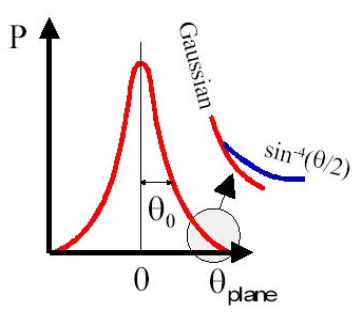
\includegraphics[width=5.0cm]{loss2}
\end{floatingfigure}
Распределение угла многократного рассеяния хорошо описывается гауссом.
При больших значениях угла, хвост распределения приближается к форме,
определённей формулой Резерфорда.

Для быстрой оценки радиационной длины можно использовать формулу:
\[
X_0\approx \frac{(716~g/cm^2)}{Z(Z+1)ln(287/\sqrt{Z})}\frac{A}{\rho},
\]
где $A, Z, \rho$ - атомный номер, атомный вес и плотность среды.

\subsection{Тормозное излучение}
\label{sec:breaking}
Заряженная частица которая движется с ускорением испускает
электромагнитное излучение, энергия которого пропорциональна квадрату
ускорения, а ускорение обратно пропорционально массе частицы. Для
тяжёлых частиц такие потери энергии ничтожно малы\footnote{Даже для
  мюона, самой лёгкой частицы после электрона, радиационные потери 40.000
  раз слабее, чем для электрона того же самого импульса \cite{kor:06}.},
другая ситуация в случае электрона. Быстрый электрон может тереть часть
энергии посредством испускания фотонов при торможении в электрическом
поле атомного ядра. Возникающие электромагнитное излучение называется
тормозным, а потери энергии частиц радиационными.

Соотношение между ионизационными и радиационными потерями энергии для
электронов можно оценить по формуле:
\[
\frac{(-\frac{dE}{dx})_{rad}}{(-\frac{dE}{dx})_{ion}} \approx \frac{E~Z}{800~MeV}
\]
Энергия при которой потери равны, называется критической, и для электронов
её можно определить из формулы $E_c \approx (800~MeV)/(Z+1.2)$ \cite{sta}.
\begin{figure}[h]\center
  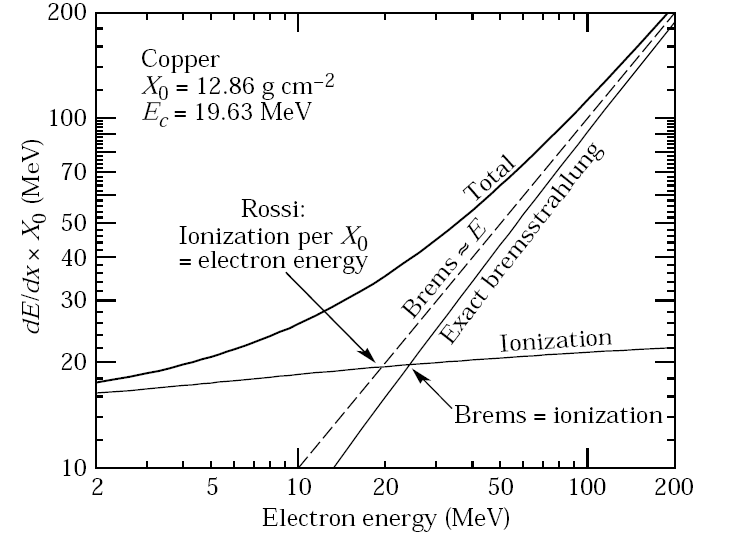
\includegraphics[scale=0.45]{loss3}
  \caption{Определение критической энергии $E_c$ электрона.}
  \label{fig:loss3}
\end{figure}

При больших энергиях электрона, когда ионизационными потерями можно
пренебречь, потери энергии на излучение можно выразить в виде:
\[
-\Bigg(\frac{dE}{dx}\Bigg)_{rad}=\frac{E}{X_0} \quad \Rightarrow \quad
E = E_0e^{-x/X_0},
\]
где $X_0$ - радиационная длинна, т.е. расстояние на котором энергия
в~результате потерь на излучение уменьшается в $e$ раз. Например, для
воздуха при нормальном давлении и температуре, радиационная длина
приблизительно 300 метров.

Видно, что высокоэнергетический электрон теряет свою энергию по
экспоненциальному закону. Однако многие фотоны испускаемые при
тормозном излучении имеют достаточную энергию для рождения
элек\-трон---позитронных пар, которые последовательно испускают фотоны
и т. д., таким образом, быстрые электроны создают так называемые
электромагнитные каскадные ливни (раздел~\ref{sec:showers}).

\subsection{Черенковское излучение}
\begin{floatingfigure}[l]{6.5cm}
  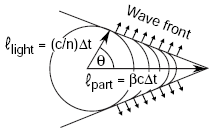
\includegraphics[width=6.0cm]{loss4}
\end{floatingfigure}
Заряженная частица, движущаяся со скоростью превышающей фазовую
скорость света в данной среде, испускает электромагнитное излучение,
называемое черенковским\footnote{излучение Вавилова---Черенка}.
Угол $\theta$ между направлением движения частицы и испускаемым
%электромагнитным %черенковским
излучением ровен $\theta =\arccos(1/n\beta)$, где $n$ - показатель
преломления вещества.
%$\cos\theta =\frac{1}{n\beta}$ где $n$ - показатель преломления среды.
%(только для $n>1$ частица может испускать данное излучение)

Этот эффект можно объяснить появлением поляризации атомов вдоль пути
движущейся частицы. Если она движется сравнительно медленно $v < c/n$,
возникающая поляризация будет распределена симметрично вокруг её пути.
Суммарное поле всех диполей равно нулю и излучения нет. Если скорость
частицы $v > c/n$, симметрия нарушается, образуется диполь и возникает
когерентное излучение.

Потери энергии на черенковское излучение учитываются формулой
Бете---Блоха (в области релятивистского возрастания), однако они
в~большинстве случаев составляют малую долю от общих потерь.
По сравнению с ионизационными потерями, их доля составляет несколько
процент. Для газов с $Z\geq7$ доля меньше чем 1\%, для лёгких газов
(He, H) приблизительно 5\% \cite{den:04}.

\subsection{Взаимодействие гамма---излучения}
Взаимодействие фотона с атомом среды приводит либо к полному поглощению
кванта, либо к существенному изменению направления его движения. Поток
фотонов с интенсивностью $I_0$ при прохождении через слой вещества
толщиной $x$ уменьшается по экспоненциальному закону:
\[
I(x)=I_{0}е^{-\mu x}.
\]
Массовый коэффициент поглощения $\mu$ связан с сечением различных
процессов взаимодействия фотонов $\sigma_i$ выражением
$\mu=\frac{N_A\rho}{A}\sum\sigma_i$, где $N_A$~-~число Авогадро,
$A$ - атомный вес и $\rho$ - плотность вещества. Сечение поглощения
$\gamma$-квантов сильно зависит от энергии фотона и представляет суммарный
вклад всех механизмов взаимодействия фотонов с веществом,
рис. \ref{fig:loss5}.
\begin{figure}[h]\center
  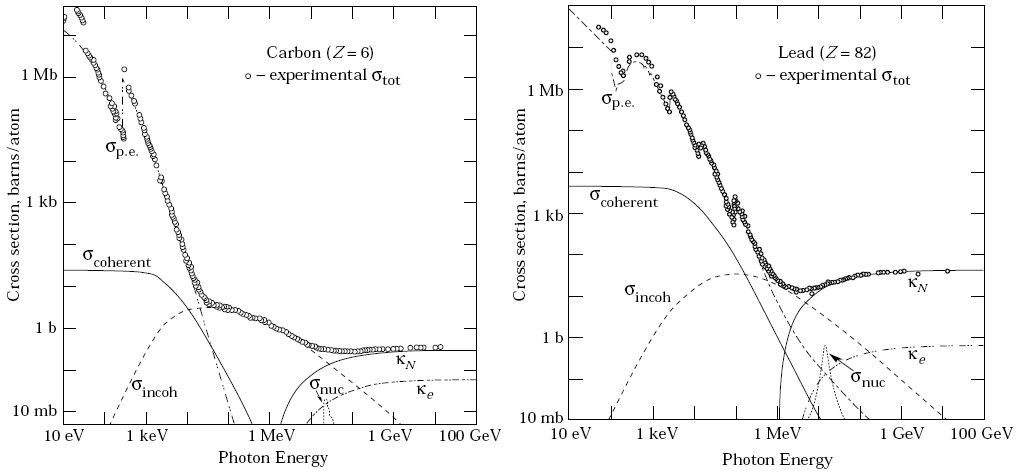
\includegraphics[scale=0.45]{loss5}
  \caption{Сечение полного поглощения фотонов с углеродом и свинцом.}
  \label{fig:loss5}
\end{figure}

Основный вклад в поглощение при низких энергиях ($E_\gamma$ < 0.1 MeV)
даёт фотоэффект, при средних энергиях (0.1 MeV < $E_\gamma$ < 10 MeV)
эффект Комптона, а~при высоких энергиях ($E_\gamma$ > 10 MeV)
преобладает процесс образования электрон---позитронных пар \cite{mas:06}.
\paragraph{Фотоэффект} процесс взаимодействия $\gamma$-кванта с связанным
электроном. Атомный электрон полностью поглощает энергию фотона, при
этом вырывается из атома. Основный вклад (80\% из полного сечение
фотоэффекта) даёт сечение на K-оболочке атома. Вероятность фотоэффекта
резко зависит от заряда атома $Z$ и энергии фотона
$\varepsilon=E_\gamma/(m_ec^2)$
\[
\sigma_{ph}\propto\frac{Z^5}{\varepsilon^3}.
\]
\paragraph{Комптон---эффект} или комптоновское рассеяние. Это рассеяние
$\gamma$-кванта на свободном электроне\footnote{Когерентное рассеяние
  фотонов на атоме как целом называется рэлеевским рассеянием. При этом
  частота излучения до и после взаимодействия остаётся неизменной.}.
Если энергия фотона существенно превышает энергию связи электрона
в атоме, можно считать электрон квазисвободным (энергией связи
пренебрегается). Энергию рассеянного фотона приобретает электрон отдачи.
Сечение комптоновского рассеяния имеет приблизительно вид
% зависит от энергии фотона и возрастает в $Z$ раз
\[
\sigma_{C}\propto Z~\frac{\ln\varepsilon}{\varepsilon}.
\]
\paragraph{Образование пар} процесс рождения электрона и
позитрона при взаимодействии $\gamma$-кванта с кулоновским полем
атомного ядра. Энергия фотона полностью передаётся образовавшимся
электрону и позитрону, а также ядру, которое получает отдачу. Однако
энергия отдачи, передаваемая ядру, обычно столь мала, что ею можно
пренебречь. Таким образом пороговая энергия образования
электрон---позитронных пар в~поле ядра\footnote{Заметим также, что
  образование $e^- e^+$ пар происходит и в кулоновским поле электрона, но
  оно сильно подавлено по сравнению с рождением пар в поле ядра.}
определяется как $E_{pair}\approx2m_ec^2$. При больших энергиях, сечение
становиться практически независимым от энергии $\gamma$-кванта, а
определяется лишь зарядом атома
\[
\sigma_{pair}\propto Z^2\ln\frac{183}{Z^{1/3}}.
\]

\subsection{Электронно---фотонные ливни}
\label{sec:showers}
Преобладающим процессом взаимодействия высокоэнергичных электронов
является тормозное излучение (раздел~\ref{sec:breaking}).
Испускаемые фотоны высоких энергии, рождают электрон---позитронные
пары.
\begin{figure}[h]\center
  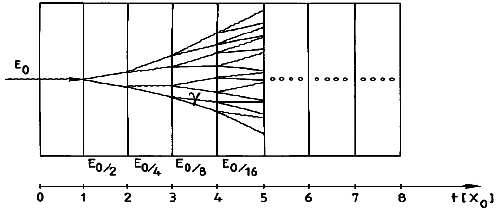
\includegraphics[height=4.4cm]{loss6}
  % \caption{Схематическое развитие электромагнитного ливня.}
  % \label{fig:loss6}
\end{figure}
Это в результате приводит к возникновению электрон---фотонных
ливней. Направление потока частиц, которые возникают, практически
совпадает с направлением первичной частицы.
%Модель развитие такого ливня показано на рис.~\ref{fig:loss6}.

Поток частиц ливня после своего образования сначала резко увеличивается.
Число частиц в ливне (сумма электронов, позитронов и фотонов) на глубине
$t$ составляет $N(t)=2^t$, где $t=x/X_0$ в единицах радиационной длины,
и энергия частицы на данной глубине равна $E(t)=E_0/2^t$. Максимальное
число частиц при развитии ливня достигается на глубине
$t_{max}=\frac{\ln E_0/E_c}{\ln2}$ и в максимуме составляет
$N_{max}\approx E_0/E_c$.

Когда энергия частиц ливня уменьшается настолько, что ионизационные
потери начинают преобладают над радиационными, ливень прекращается.
Значение энергии, когда она становится критической, можно выразить
как $E_c=E_0/2^{t_{max}}$ \cite{kor:06}.

Отмеченные закономерности существенны при конструкции калориметров,
которые можно использовать при измерении энергии электронов и фотонов
в экспериментах с частицами высоких энергии.

\subsection{Взаимодействие нейтронов с веществом}
Нейтроны взаимодействуют с веществом в основном за счёт их взаимодействия
с атомными ядрами посредством ядерных сил\footnote{Сечение
  электромагнитного взаимодействия нейтрона, эффект от взаимодействия
  магнитных моментов нейтрона и атомного электрона, приблизительно
  в~$10^6$ раз меньше, чем для электрона (за исключением, когда эффект
  происходит в ферромагнетиках).}. Поэтому регистрация нейтронов связана
с взаимодействием при котором сначала должны образоваться ионизирующие
частице.
\begin{floatingfigure}[l]{3.9cm}
  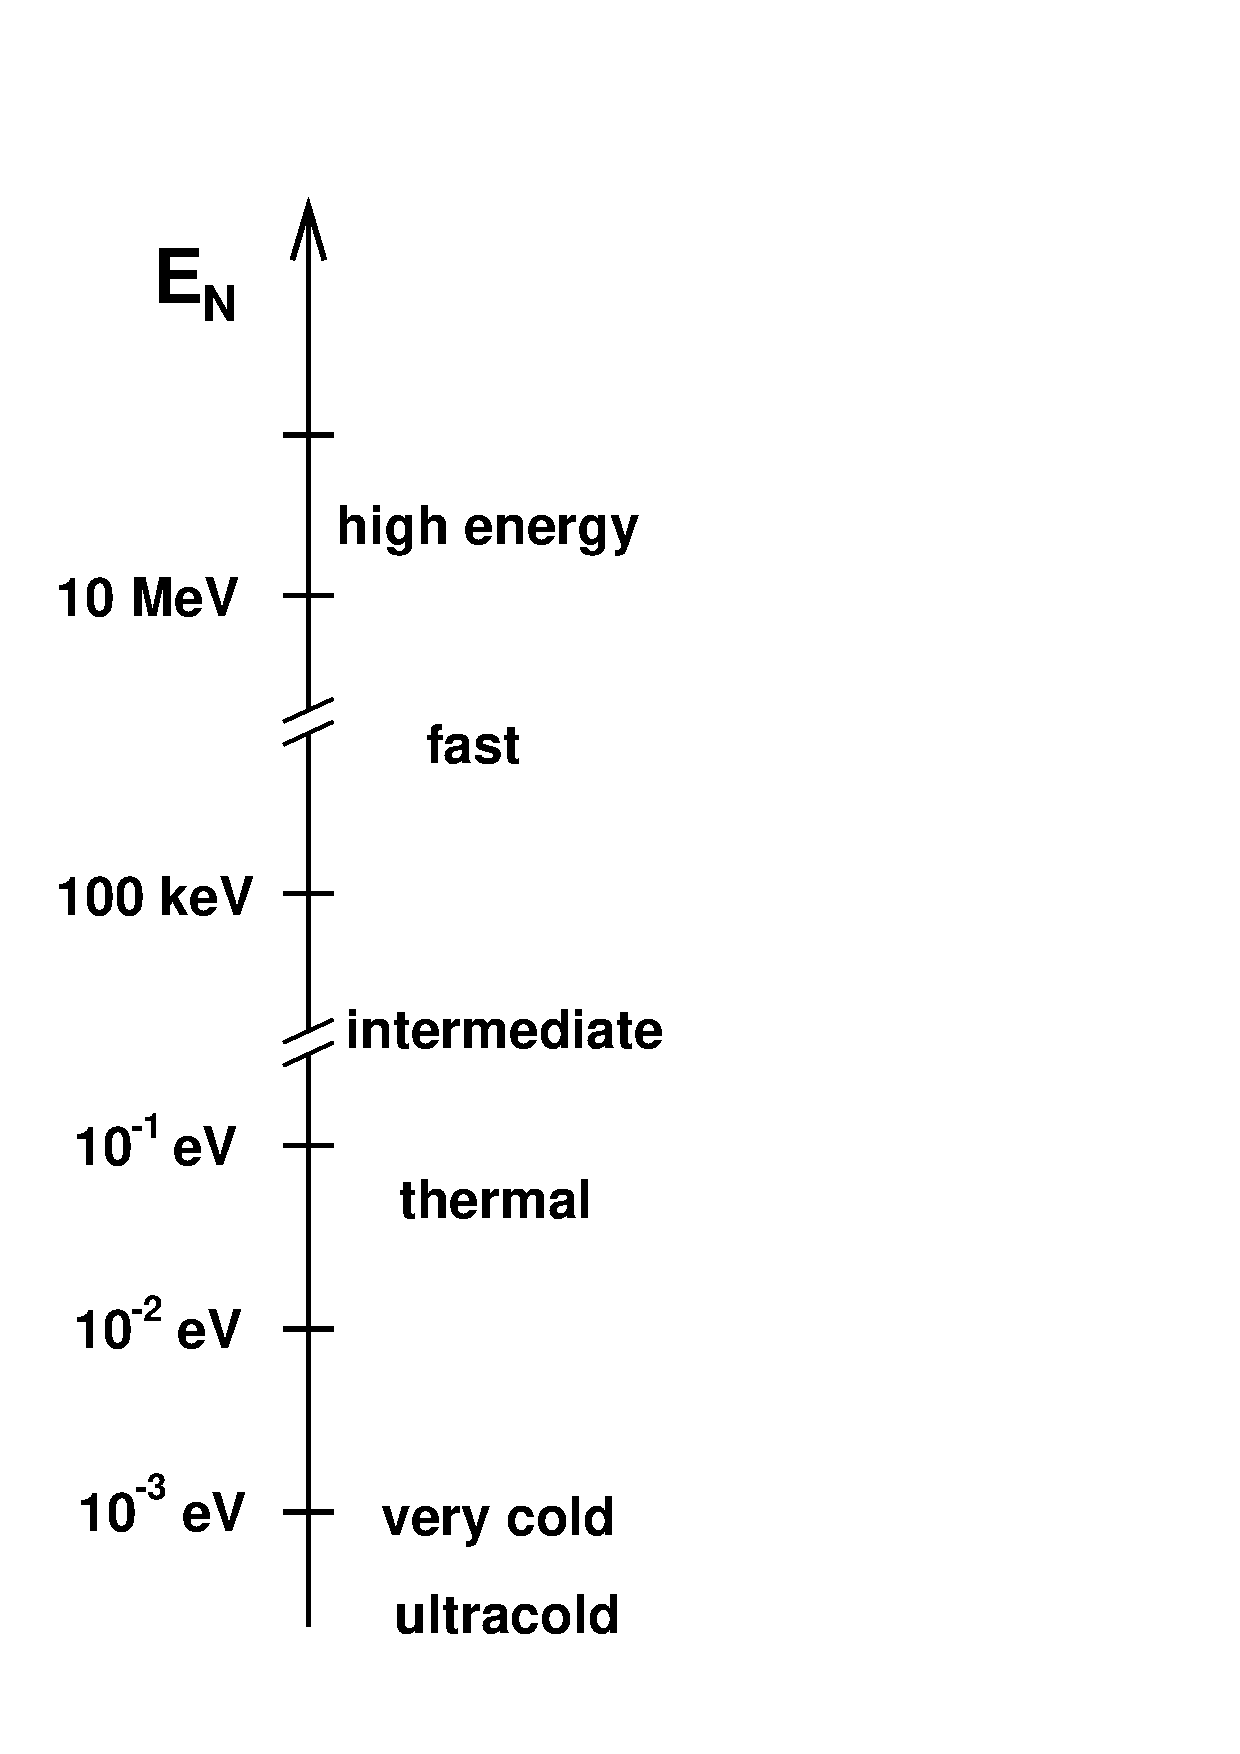
\includegraphics[width=3.1cm]{loss7}
\end{floatingfigure}
\hspace{-0.3cm}
Сечение взаимодействие нейтронов с веществом сильно зависит от энергии
нейтрона. Условно принято называть нейтроны с энергиями в интервале
от 0 до 100 keV, медленными. Если энергия выше, это быстрые нейтроны.
Медленные нейтроны ещё принято разделить на несколько интервалов:
ультрахолодные (самые низко энергичные), холодные, тепловые  и так
называемые промежуточные. Для нейтронов того или иного энергетического
интервала, следует применять разные методы регистрации \cite{kal:66}.

В зависимости от того, попадает нейтрон в ядро или нет, можно разделить
его взаимодействие с ядром на две группы: \clearpage
\paragraph{упругое рассеяние} без проникновения частицы
в~ядро (потенциальное рассеяние на силовом поле ядра). Ядро отдачи
приобретает кинетическую энергию и сможет ионизировать в~среде.
\paragraph{разнообразные ядерные реакции:} радиационный захват
(n, $\gamma$), реакции с~образованием одной или нескольких частиц (n, p),
(n, $\alpha$), неупругое рассеяние, упругое рассеяние при котором нейтрон
заходит в~ядро (резонансное рассеяние), деление ядер и т. п. Как правило,
эти реакции сопровождаются вылетом из ядра быстрых заряженных частиц,
которые могут в~веществе создать ионизационные эффекты.
\vspace{5.0cm}
\begin{figure}[h]\center
  \hspace*{-0.5cm}
  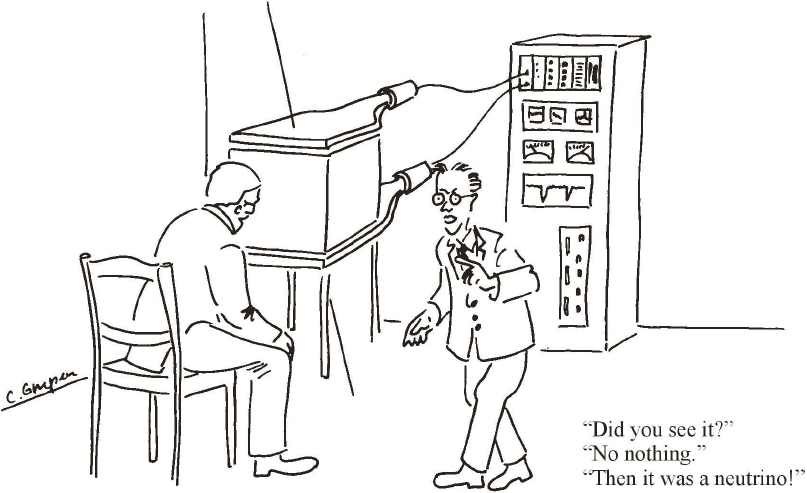
\includegraphics[width=15.0cm]{loss_last}
\end{figure}



%%% Local Variables:
%%% TeX-master: "referat"
%%% End:
